\documentclass[10pt]{beamer}
\usetheme{Warsaw}
\usepackage[T1]{fontenc}
\usepackage[utf8]{inputenc}
\usepackage{chronosys}
\usepackage{graphicx}
\usepackage{hyperref}
\usetheme{shadow}
\useinnertheme{circles}
\setbeamertemplate{caption}[numbered]
\usecolortheme[named=gray]{structure}
%----------------------------------------------------------------------------------------
%	PRESENTATION INFORMATION
%----------------------------------------------------------------------------------------
\title{ScimBa Feel++}
\subtitle{CSMI1}
\author{ Helya Amiri \\ Rayen Tlili }
\institute[]{University of Strasbourg \\ \smallskip}
\date[\today]{Mathematics and applications \\ \today}

\begin{document}
%----------------------------------------------------------------------------------------
%	TITLE SLIDE
%----------------------------------------------------------------------------------------
\frame{\titlepage}
\begin{frame}
    \tableofcontents
\end{frame}

% Partie 1: Introduction
\section{Introduction to the project}
\begin{frame}
    \frametitle{Introduction}
    This project aims for the coupling of ScimBa and Feel++. This involves integrating the capabilities of both tools. 
    \\This integration would allow users to leverage the advanced features of each of these libraries and use them synergistically to solve complex problems.
\end{frame}


% Partie 2: 
\section{Presentation of the libraries}
\begin{frame}
    \setbeamertemplate{blocks}[rounded][shadow=false]
    \frametitle{ScimBa}
    \framesubtitle{ gathers tools for scientific machine learning, mainly focusing on solving partial  \\  differential equations (PDEs) and related tasks in scientific computing.}

    \begin{itemize}
        \item ScimBa blends machine learning with scientific computing. 
        
        %This integration helps researchers create advanced models and algorithms for solving tough scientific problems.

        \item ScimBa offers PDE solvers as a core feature. 
        
        %These solvers are crucial for studying physical processes like fluid dynamics, heat transfer, and quantum mechanics.
    \end{itemize}
\end{frame}

\begin{frame}
    \setbeamertemplate{blocks}[rounded][shadow=false]
    \frametitle{Feel++}
    \framesubtitle{is a C++ implementation that combines Galerkin methods, including finite element and \\spectral element methods, to tackle partial differential equations across 1D, 2D, and 3D domains.}

    \begin{itemize}
        \item Feel++ includes toolboxes for solving physics-based problems like fluid mechanics, solid mechanics, and heat transfer.
        
        % These toolboxes provide pre-built applications and libraries for solving specific types of problems.
        
        \item  provides a Python interface (pyFeel++) for manipulating mathematical objects and solving PDEs with Python. 
        
        %This provides flexibility and interoperability with other Python-based libraries and tools. 
        
    \end{itemize}
\end{frame}


% Partie 3:

\section{Approach}

\begin{frame}
    \setbeamertemplate{blocks}[rounded][shadow=false]
    \frametitle{Coupling}
    \begin{block}{Tight Coupling}
    Modules are highly dependent on each other. Changes in one module often require corresponding changes in other modules.

    %This type of coupling can make the codebase rigid and difficult to maintain, as modifications in one part of the code may have unintended consequences elsewhere..
    \end{block}

    \begin{block}{Loose Coupling}
    Modules are relatively independent and have minimal dependencies on each other.

    %This type of coupling promotes modularity and flexibility, as changes in one module are less likely to affect other modules.

    \end{block}
\end{frame}


% Partie 4:

\begin{frame}
    \setbeamertemplate{blocks}[rounded][shadow=false]
    \frametitle{Starting Points}
    \textbf{Objective:}

    %Implement loose coupling between ScimBa and Feel++ to leverage the strengths of both libraries effectively.

    \begin{itemize}
        \item Analyze ScimBa and Feel++ functions to find integration points.
        
        % Determine where the two libraries can interact with minimal dependencies, promoting loose coupling.

        \item Use Feel++ for simulations and scientific computing to create diverse datasets.
        
        % Implement methods to inject data generated by Feel++ into ScimBa's machine learning algorithms. 

        \item Establish clear interface and protocols for seamless communication between libraries.
        
        %Verify that the loose coupling approach allows for seamless communication and interoperability between the two libraries.
        
    \end{itemize}   

\end{frame}


% Partie 5:

\begin{frame}{Roadmap}
    \begin{center}
        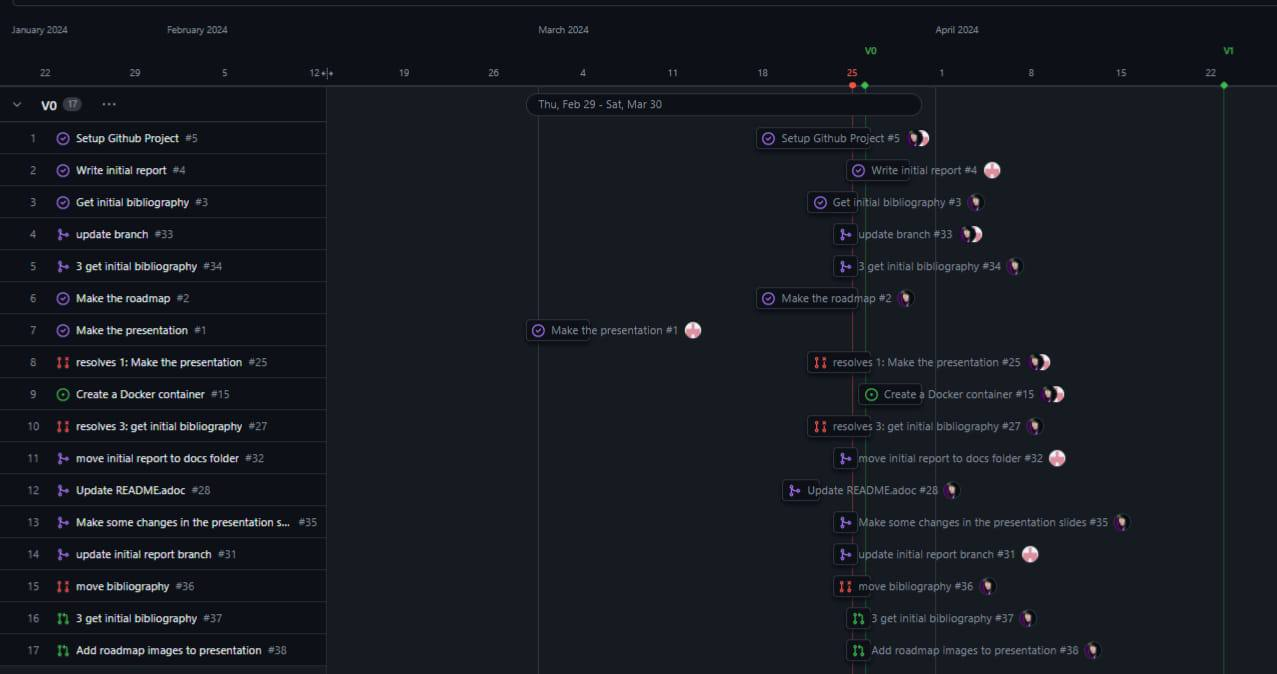
\includegraphics[width=0.7\textwidth]{images/roadmap1.png}
        \vspace{1em} % Ajoute un espace vertical
        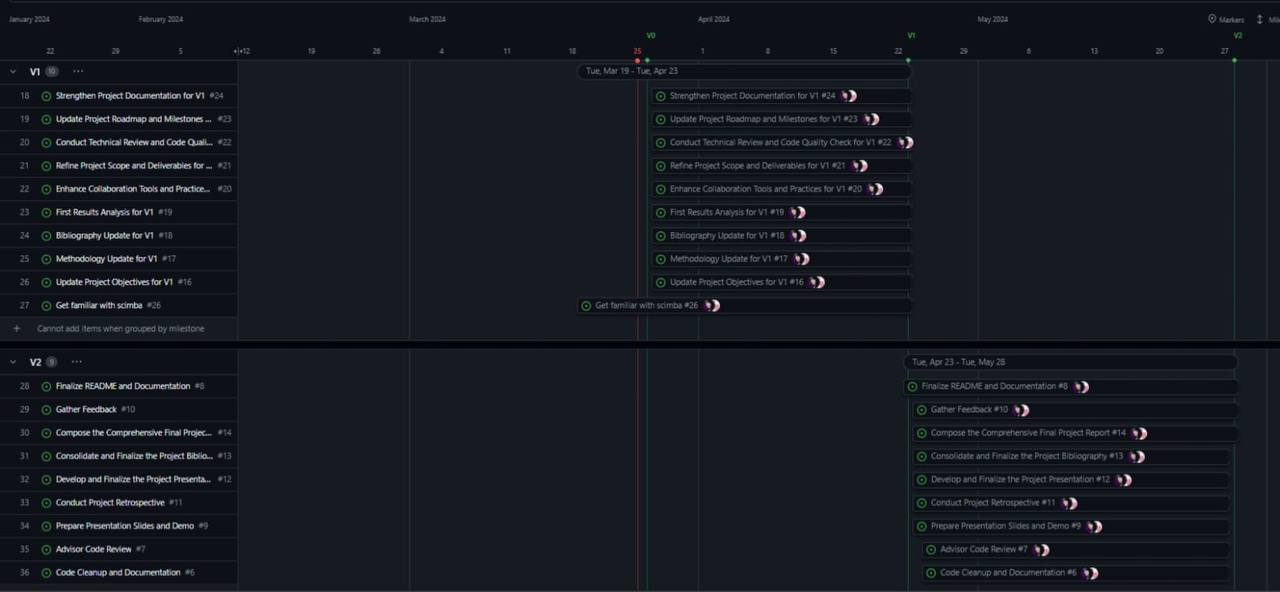
\includegraphics[width=0.7\textwidth]{images/roadmap2.png}
    \end{center}
\end{frame}

% Partie 6:

\section{References}
\begin{frame}
    \setbeamertemplate{blocks}[rounded][shadow=false]
    \frametitle{References}
    \begin{itemize}
    
        \item \href{https://docs.feelpp.org/user/latest/index.html}{Feel++ Documentation}
        
        \item \href{https://sciml.gitlabpages.inria.fr/scimba/}{ScimBa Documentation}

        \item \href{https://en.wikipedia.org/wiki/Coupling_(computer_programming)}{Coupling}
            
    \end{itemize}
\end{frame}


\end{document}
